\documentclass{ercisbeamer}

\title{Mental Models}
\subtitle{Effective Studying}
\author{Sven Ligensa}
\institute{European Research Center for Information Systems (ERCIS)}
\date{\today}


\begin{document}

\setbgimage{00_resources/jungle_brain}
\begin{frame}
    \begin{tbox}
        \titlepage
    \end{tbox}
\end{frame}
\setbgimage{}

\begin{frame}{Contents}
    \tableofcontents
\end{frame}

\section{Overview}
\begin{frame}{Overview}
    \begin{tbox}
        \begin{itemize}
            \item \red{\textbf{Deeply entrenched and highly efficient skills or knowledge structures}}
            \begin{itemize}
                \item Interrelated concepts \grey{(or sequence of motor skills)}
                \item \red{Connected}: Fused into \red{meaningful whole} and 
            \end{itemize}
            \item Mental representation of (key ideas/underlying principles/rules from) external reality (learning material)
            \begin{itemize}
                \item Differentiate: Salient concepts vs. Unimportant details
            \end{itemize}
            \item Arise and improve through \red{effortful practice}
            \item Important: Ability to discern when our mental models are \negative{not} working
            \item Conscious or subconscious
            \item Connected with other mental models (prior knowledge)
            \item Adaptability and applicability in various circumstances
            \item Metaphors can deliver structure to build mental model
        \end{itemize}
    \end{tbox}
\end{frame}

\begin{frame}{Overview}
    \begin{tbox}
        \begin{itemize}
            \item Good: Put new knowledge in wider \red{context}
            \begin{itemize}
                \item E.g. learning an \red{abstraction} or grounding it in something \red{concrete}
                \item Give meaning to what you learn
            \end{itemize}

            \vspace{1em}
            
            \item My experience: Connecting information from different contexts is \red{fun}
            \begin{itemize}
                \item E.g. Insight that ``Faltung'' \grey{(German word, Statistics)} is just a translation of ``Convolution'' \grey{(English word, DL)} $\Rightarrow$ Same computation
            \end{itemize}
        \end{itemize}
        \vspace{-.8em}

        \begin{figure}
            \centering
            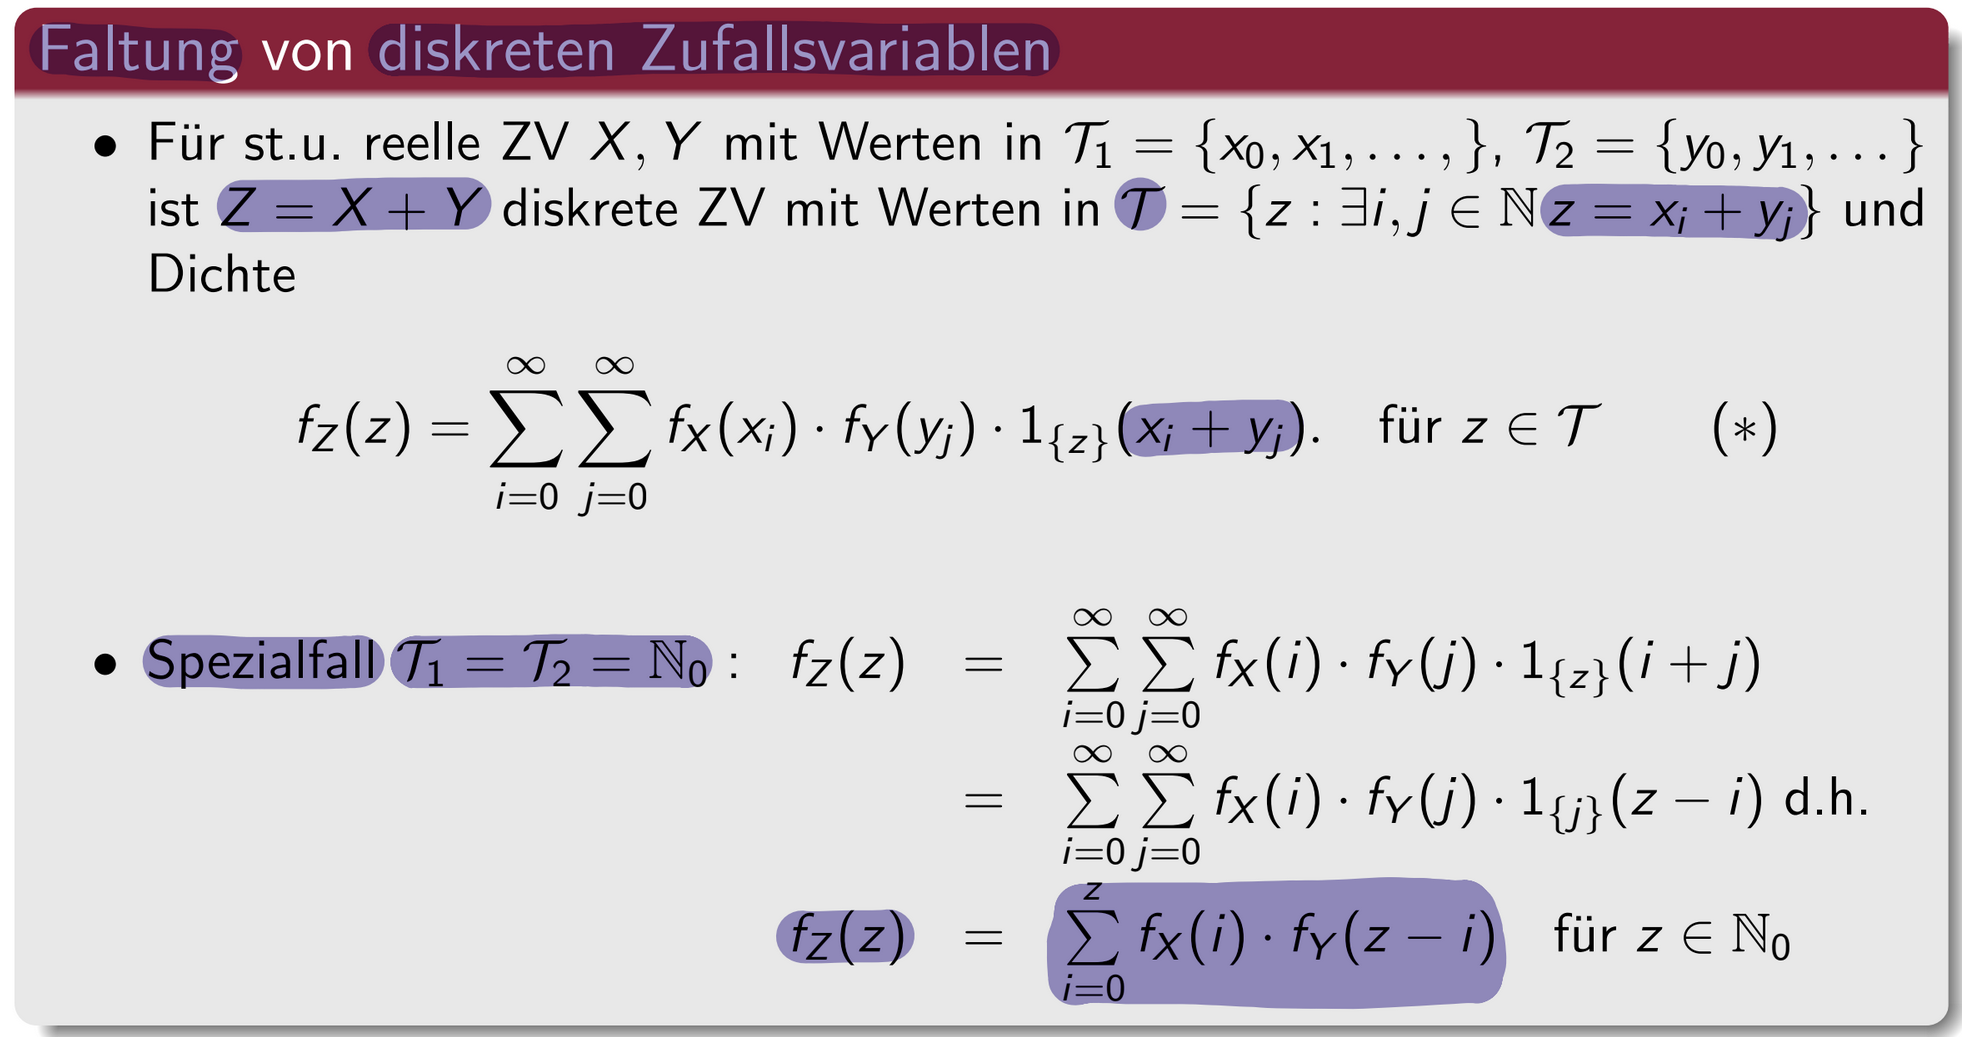
\includegraphics[height=.4\paperheight]{10_resources/da_conv.png}
            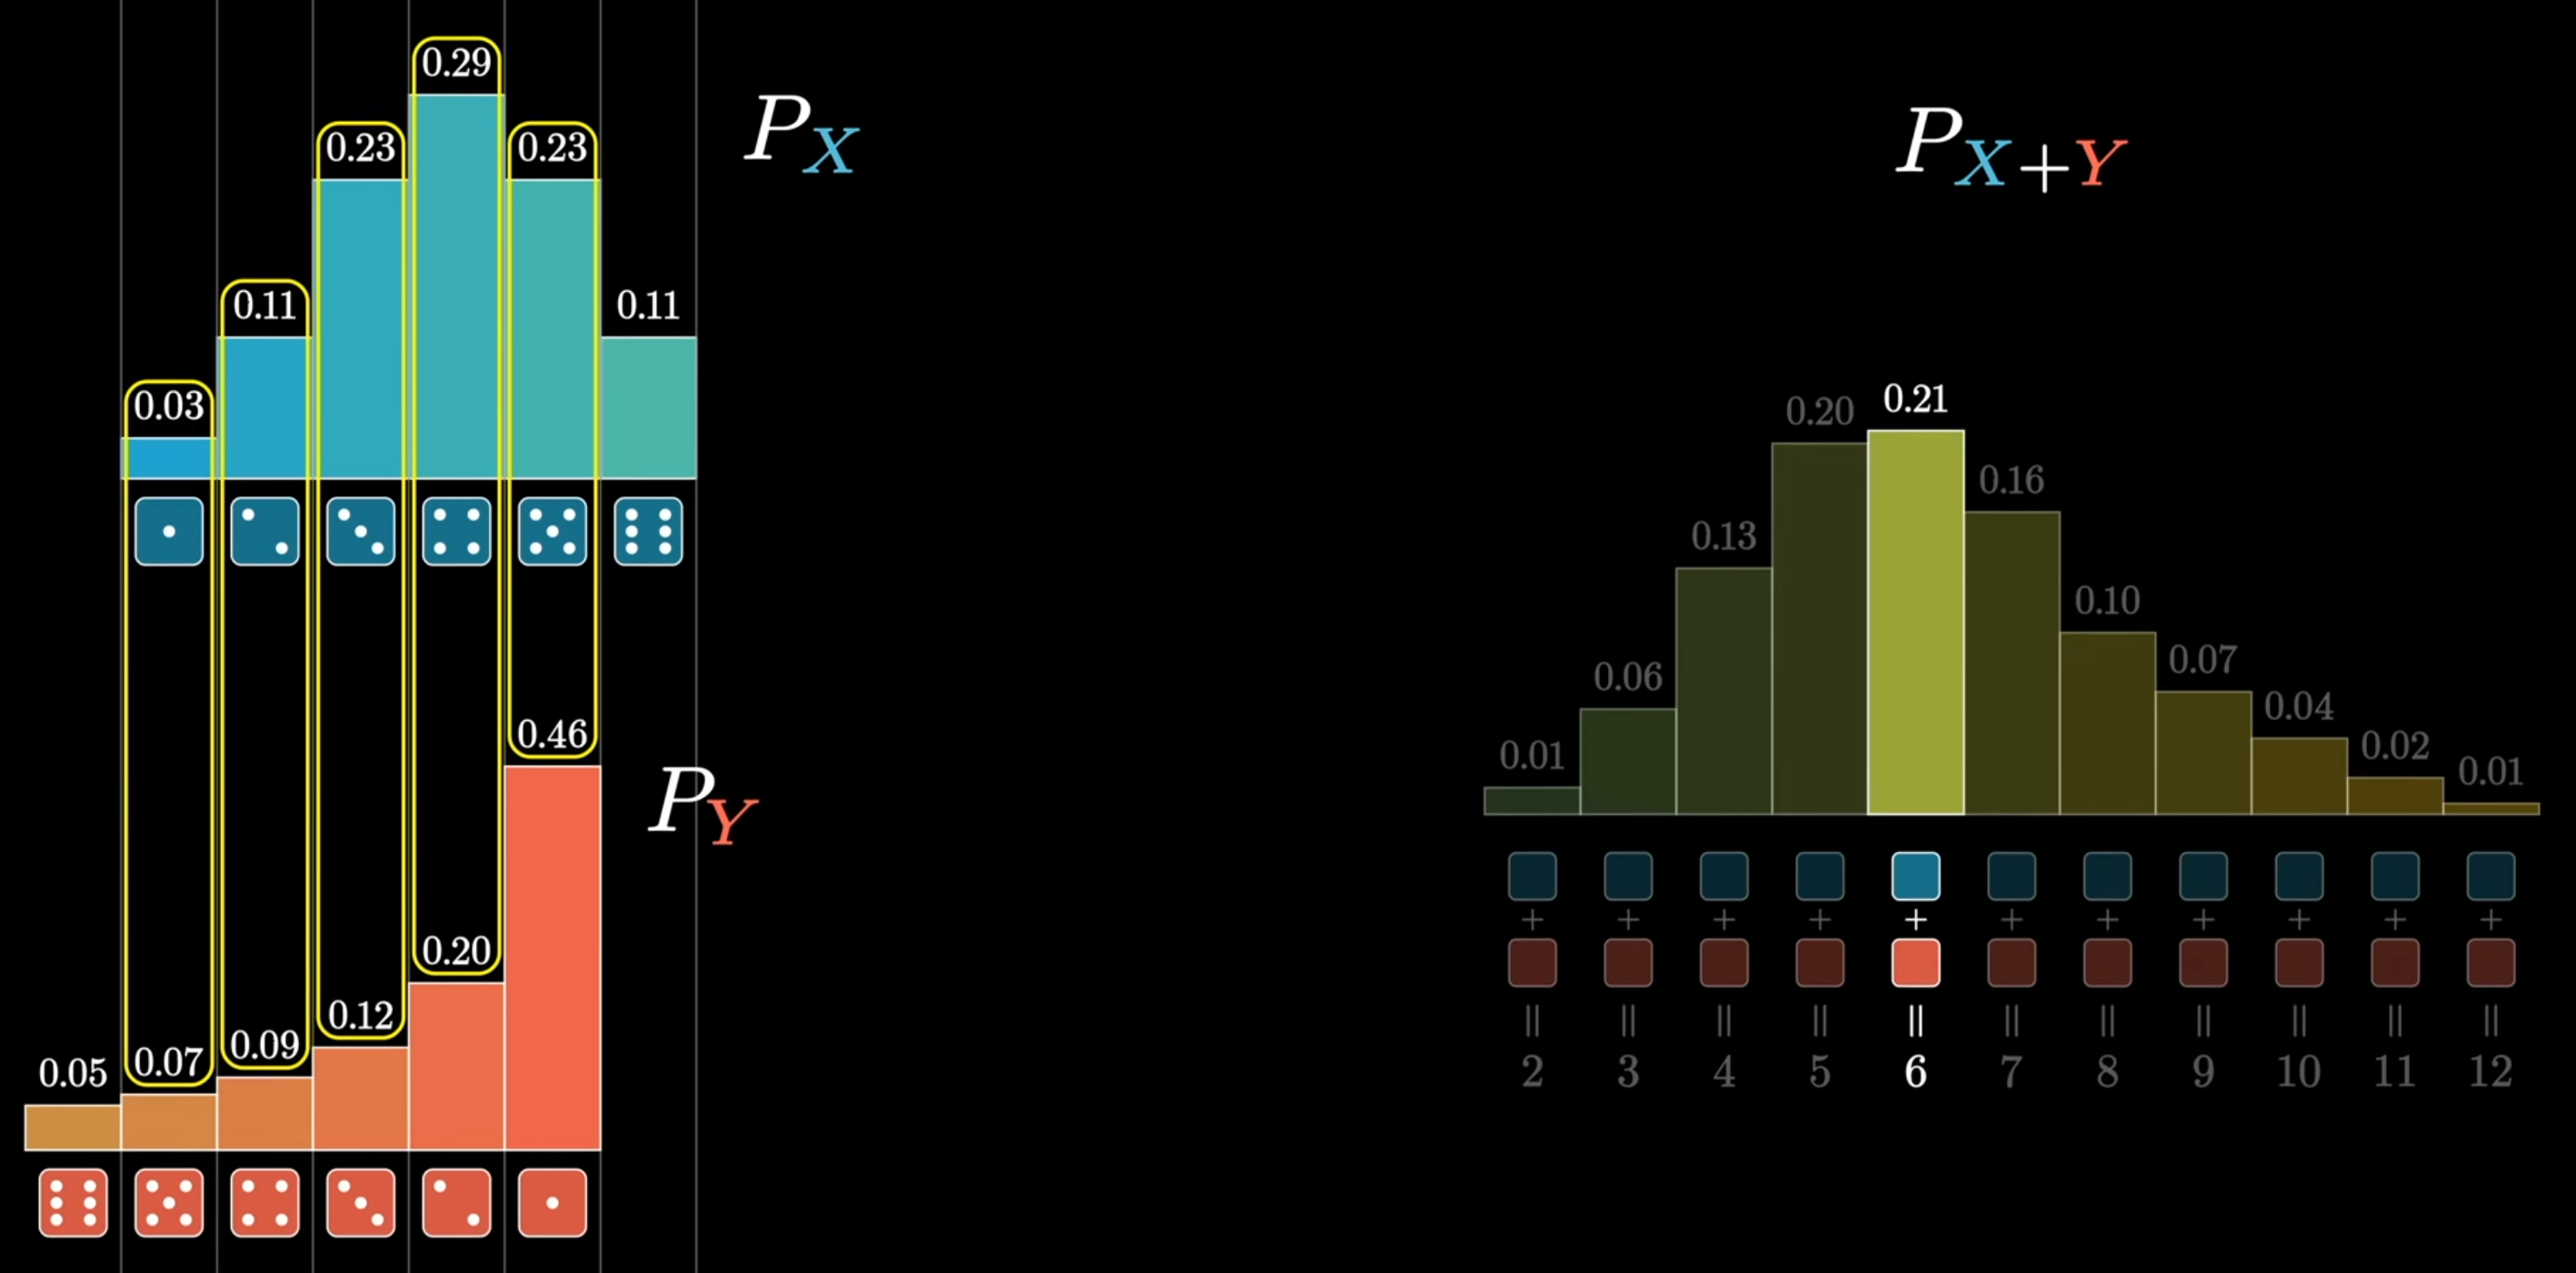
\includegraphics[height=.4\paperheight]{10_resources/3b1b_conv.png}
            \vspace{-0.5em}
            \caption{\small{\emph{Left}: Slides from DA, \hspace{.8em} \emph{Right:} \url{https://youtu.be/KuXjwB4LzSA?feature=shared&t=452}}}
        \end{figure}
        
    \end{tbox}
\end{frame}

\setbgimage{10_resources/syntax_semantics}
\section{Syntax $\ne$ Semantics}
\begin{frame}{Syntax $\ne$ Semantics}
    \begin{tbox}
        \begin{itemize}
            \item \red{Essence} of something usually \red{\textbf{not in syntax}}
            \begin{itemize}
                \item Precise wording usually irrelevant
            \end{itemize}
            \item Mastering lecture $\ne$ Mastering ideas behind it
                \begin{itemize}
                    \item[$\rightarrow$] Implications for lecture and exam design!
                \end{itemize}
            \item Nevertheless: Terminology (e.g. Latin names) can be very helpful to remember characteristics
        \end{itemize}
    \end{tbox}
\end{frame}

\setbgimage{10_resources/mental_model}
\section{Analogies \& Examples}
\begin{frame}{Analogies \& Examples}
    \begin{tbox}
        \begin{itemize}
            \item Map, framework
            \item \red{Code library}: Library of myriad useful solutions that we can call on at will
        \end{itemize}
    \end{tbox}

    \vspace{.5em}

    \begin{tbox}
        \begin{itemize}
            \item \emph{Can you think of examples?} \pause
            \begin{itemize}
                \item Motor skills
                \begin{itemize}
                    \item Driving a car
                    \item Typing on a keyboard
                    \item Hitting a ball with a racket
                    \item Performing a muscle up
                \end{itemize}
                \item Cognitive skills
                \begin{itemize}
                    \item Knowing a topic inside out and being able to reference it a will (e.g. knowing characteristics of a process or how parts of a complex system interact with each other)
                \end{itemize}
            \end{itemize}
        \end{itemize}    
    \end{tbox}
\end{frame}

\setbgimage{10_resources/outline}
\section{Make the Material Your Own}
\begin{frame}{Make the Material Your Own}
    \begin{tbox}
        \begin{itemize}
            \item Actively \red{question} the \red{structure} of the presented material and \red{restructure} it as needed (also overarching multiple lecture sessions or even modules)
            \begin{itemize}
                \item It may be the most logical for the lecturer, but not for you
                \item Everybody thinks a bit differently
                \item They may be impacted by the \emph{Curse of Knowledge}
                \item After all, it has to make sense for \emph{you}
            \end{itemize}
        \end{itemize}
    \end{tbox}
\end{frame}
\setbgimage{}

\section{Advantages}
\begin{frame}{Advantages}
    \begin{itemize}
        \item More successful at \positive{selecting right solution} for unfamiliar problems
        \begin{itemize}
            \item Extremely important for knowledge workers
            \item In current times: While AI tools \grey{(like ChatGPT)} can aid with many retrieval tasks, they will not be able to replace your mental models \grey{(in the foreseeable future)}
        \end{itemize}
        \item Results in \positive{conceptual knowledge} ($=$ understanding relationships of of basic elements within larger structure) instead of factual knowledge
    \end{itemize}
\end{frame}

\setbgimage{10_resources/big_picture}
\section{Implementation}
\begin{frame}{Implementation}
    \begin{tbox}
        \begin{itemize}
            \item Distill information into ``\red{Big Picture}''
            \begin{itemize}
                \item \grey{(Helps me personally a lot)}
                \item Contains overview, interrelation of topics, general insights
                \item May not be directly relevant to exam, but very relevant for general understanding
                \begin{itemize}
                    \item \emph{How often have you been asked (by a relative or friend) about what a course is about and were not really able to communicate it clearly?}
                \end{itemize}
                \item Serves as polished reference for later
                \item Like a conceptual entry point to retrieve more detailed knowledge
                \item Refine iteratively during the semester (and possibly even later)
            \end{itemize}
            \item Test yourself on key concept
            \begin{itemize}
                \item Be able to \red{define} it (in own words) and \red{use} it
            \end{itemize}
        \end{itemize}
    \end{tbox}
\end{frame}
\setbgimage{}

\begin{frame}{Example ``Big Picture'' created by me}
    \centering 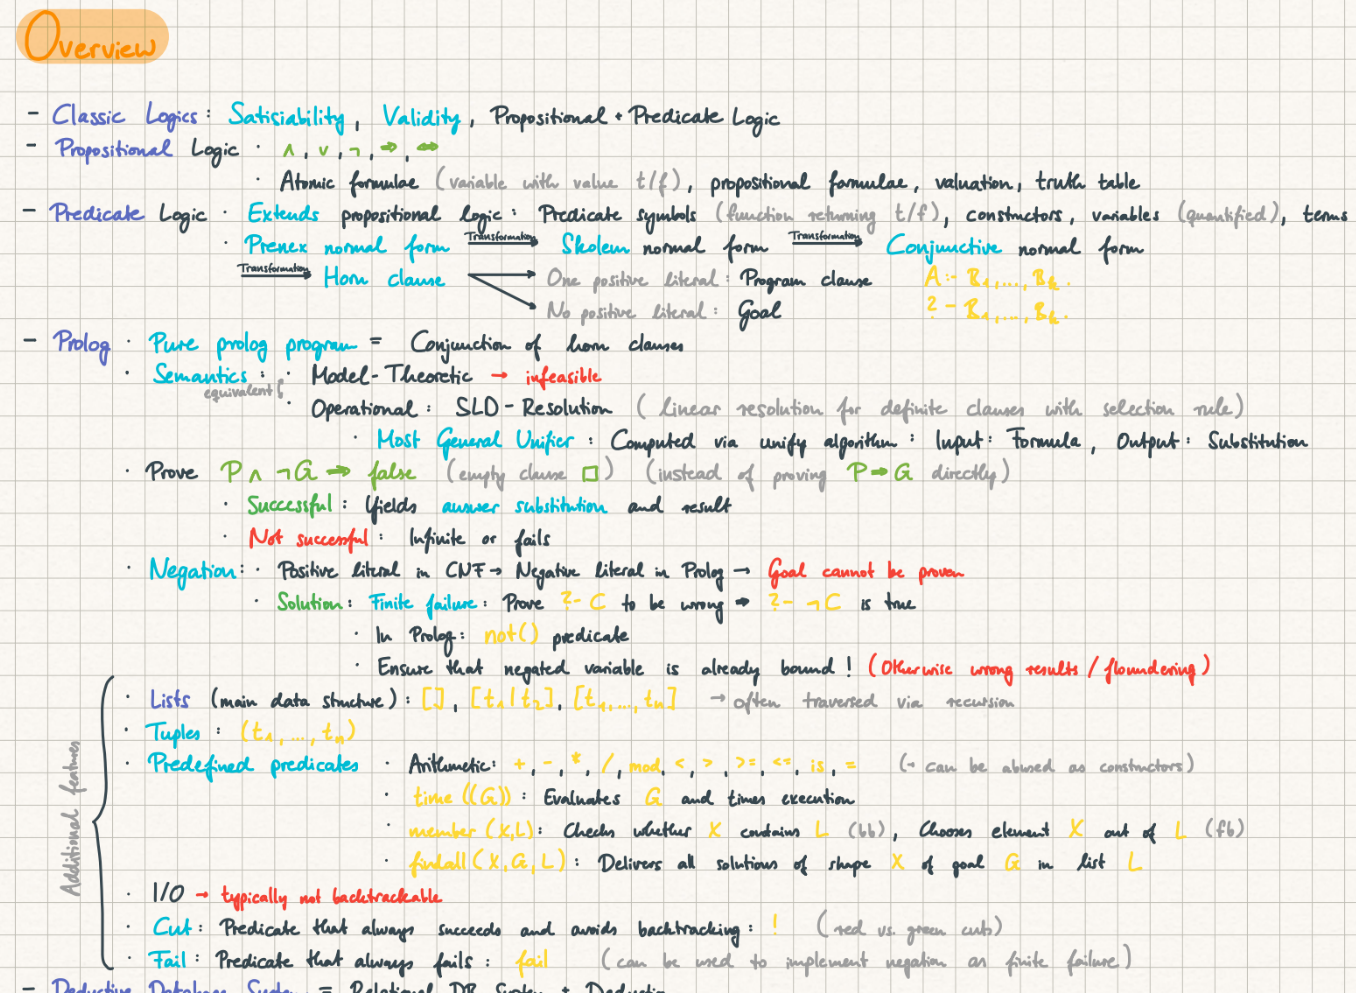
\includegraphics[height=.83\paperheight]{10_resources/big_picture_lsp_example.png}
\end{frame}

\section{Now You!}
\begin{frame}{Now You!}
    \begin{itemize}
        \item \emph{Which of your courses benefit most from creating Mental Models?}
        \item \emph{Do you want to create Big Pictures? Or do you think other methods can be more efficient?}
        \item \emph{How---if at all---can you effectively combine the Big Picture and Retrieval?}
    \end{itemize}
\end{frame}

\chapteroverview{10}

\thankyou{Happy Learning!}{sven.ligensa@uni-muenster.de}

\sources

\end{document}
